%\documentclass[pra,showpacs,twocolumn]{revtex4}


\documentclass[preprint,12pt]{article}
%%%%%%%%%%%%%%%%%%%%%%%%%%%%%%%%%%%%%%%%%%%%%%%%%%%%%%%%%%%%%%%%%%%%%%%%
\usepackage{amssymb}
\usepackage{amsmath}
\usepackage{graphicx}
%\usepackage{multirow}
%\usepackage{gensymb}
\usepackage{float}
%\usepackage{authblk}
%\setcounter{MaxMatrixCols}{10}

\begin{document}

\title{Ionization of molecules by multicharged bared ions by using the
stoichiometric model}
%\author{author}
%\affiliation{Consejo Nacional de Investigaciones Cient\'{\i}ficas y
%T\'{e}cnicas - Universidad de Buenos Aires, Instituto de
%Astronom\'{\i}a y F\'{\i}sica del Espacio, Pabell\'on IAFE, 1428 Buenos Aires, Argentina;}

\date{\today }

\maketitle

\begin{abstract}
\end{abstract}

%\pacs{79.20.Rf, 68.49.Bc, 34.20.Cf,34.50.-s,34.35.+a}



\subsection{Scaling rule}

\subsubsection{Toburen numbers}

The first attempt to develop a comprehensive but straightforward
phenomenological model for electron ejection from large molecules was
proposed by Toburen {\it et al.}~\cite{toburen1975,toburen1976}.
The authors found it convenient to scale the experimental ionization
cross section in terms of the number of outer or weakly bound valence
electrons \textbf{(i.e. total number of electrons minus the K-shell)}.
\textbf{Following Toburen we can define the ionization} cross section per weakly bound electron
%or ionization cross section per valence electron,
$\sigma_{e}^T$, as
\begin{equation}
\sigma_{e}^T=\frac{\sigma_{M}}{N_{M}}=\frac{\sum\limits_{\alpha}
n_{\alpha} \sigma_{\alpha}}{\sum\limits_{\alpha}n_{\alpha}\nu_{\alpha}^T}
=\sigma_{e}(v)\,,
\label{27}
\end{equation}
where \textbf{$\nu_{\alpha}^T$ are the Toburen numbers for each atom:}
\begin{equation}
\nu_{\alpha}^T=\left\{
\begin{array}{ll}
1, & \text{H,} \\
4, & \text{for C,} \\
5, & \text{for N and P,} \\
6, & \text{for O and S,}
\end{array}\right.
\label{eq:nelec}
\end{equation}
%and $\nu_{\text{H}}=1$.
The Toburen rule can be stated by saying that
$\sigma_{e}$ is a \textit{universal} parameter independent on the
molecule, which depends solely on the impact velocity\textbf{
, and holds for high impact energies (i.e. 0.25-5 Mev/amu).}
%In Ref.~\cite{toburen1976}, it was found experimentally that for proton
%impact on some simple molecules, $\sigma_{e}$ results
%\begin{equation}
%\begin{array}{cccc}
%E\text{(MeV)}               & 0.25 & 1.00 & 2.00 \\
%\sigma_{e} (10^{-16}cm^{2}) & 0.39 & 0.17 & 0.11
%\end{array}
%\label{30}
%\end{equation}
%with an estimated error of about 20\%.

\textbf{
These $\nu_{\alpha}^T$ can be interpreted as the number of active 
electrons in the collision. Of course, at very high energies also de 
K--shell electrons will be ionized and these numbers will be different. }

A similar \textbf{dependence with the number of weakly bound electrons} was found in
Ref.~\cite{itoh2013} for proton impact on uracil and adenine.


Figure 4a shows \textbf{our CDW results for} $\sigma_{e}^T$ as a function of
the impact velocity for different projectile charges computed with the
SSM for the sixteen molecular targets displayed in
Table~\ref{tab:families}. The universality with $Z$ is the one provided
by Born approximation, i.e., $\sigma _{e}^T(Z)=Z^{2}\sigma_{e}^T(Z=1)$,
and it holds for large impact velocities, as shown Figure 4a.
Of course, for lower impact velocities, the CDW breaks the behavior of
the $Z^{2}$ rule.

Although the Toburen \textbf{scaling} holds for high energies,
its performance is still not satisfactory: the universal band is quite
broad.


\subsubsection{New scaling}

The departure of our theoretical
results from the Toburen rule can be explained by %the fact that
%our atomic cross sections $\sigma_{\alpha}$ behave differently for
%each atom in terms of the projectile charges. By
\textbf{inspecting Figure 1. It can be noted}
 that the rule $\sigma_{\alpha}/\nu_{\alpha}^T\sim
\sigma_{e}^T$ \textbf{approximatelly constant} is not well satisfied by 
the CDW model.
\textbf{
For example, Figure 1 shows that the cross sections for O are actually 
very similar to the cross sections for C, suggesting 4 active electrons 
in O instead of 6. In the same way the number of active electrons for
N, P and S are also different from the $\nu_{alpha}^T$ in Equation 
(\ref{eq:nelec}). This will be an important change in the scaling for 
molecular targets. Based on the CDW results we propose a new scaling 
given by}
%A much better general atomic rule is given by
\begin{equation}
\sigma_{e}^{\text{CDW}}=\frac{\sum\limits_{\alpha}
n_{\alpha}\sigma_{\alpha}^{\text{CDW}}}{\sum\limits_{\alpha}n_{\alpha}
\nu_{\alpha}},
\label{32}
\end{equation}
\textbf{where $\nu_{\alpha}$ are the new numbers of active electrons per 
atom obtained from the CDW ionization cross sections for different ions 
in H, C, N, O, P , and S targets. The new values are
\begin{equation}
\nu_{\alpha}=\left\{
\begin{array}{ll}
1, & \text{H,} \\
4, & \text{for C, N, O} \\
4.5, & \text{for P, S} \\
\end{array}\right.
\label{eq:scalingCDW}
\end{equation}
}
The \textbf{scaled} cross sections
$\sigma_{e}^{\text{CDW}}$ are plotted in Figure~4b. A much better sharp
band is observed, especially \textbf{for impact energies $E=(0.5-8)MeV/amu$ 
for $Z=1$ and $Z=2$; and $E=(2.5-8)MeV/amu$ for $Z>2$.}
%at high energy, where the theory is expected to work.
\textbf{
The experimental data for ionization of adenine, cytosine, thymine, 
guanine, uracil, pyrimidine and THF by proton impact seems to 
corroborate the new scaling. It will be interesting to cross-check for 
experiments with projectile charge states $Z>1$.}

\textbf{In table \ref{nn} we display the number of active electrons 
obtained using the present scaling for some molecules of interest. These 
numbers are very different from those proposed by Toburen \cite{} and 
used by other authors \cite{Itoh,others}.}


\begin{table}
\begin{center}
\begin{tabular}{llllll}
\hline
 Molecule & number &Molecule         &number & Molecule             &number \\
 H$_2$    & 2  & C$_2$H$_7$N         & 19    & C$_4$H$_5$N$_3$O     & 37    \\
 H$_2$O   & 6  & C$_4$H$_8$O         & 28    & C$_5$H$_6$N$_2$O$_2$ & 42    \\
 NH$_3$   & 7  & C$_4$H$_4$N$_2$     & 28    & C$_5$H$_5$N$_5$      & 45    \\
 CH$_4$   & 8  & C$_6$H$_6$          & 30    & C$_5$H$_5$N$_5$O     & 49    \\
 CH$_5$N  & 13 & C$_4$H$_4$N$_2$O$_2$& 36    & C$_5$H$_{10}$O$_5$P  & 54.5  \\
 \hline
\end{tabular}
\caption{New scaling numbers for SOME molecular targets of biological interest.}
\label{nn}
\end{center}
\end{table}

\textbf{An alternative way of showing this scaling is to plot the ionization cross sections of molecules as a function of the number of active electrons given in table \ref{nn}. This is displayed in the figure \ref{recta} for impact energies 0.5, 1 and 2 MeV. As can be noted the CDW ionization cross sections calculated for different molecules actually show a linear dependence with the number of electrons given in table \ref{nn}. We obtain similar straigth lines even for E=10 MeV. The comparisson with the experimental data available shows very nice agreement from the smallest molecules H$_2$, H$_2$O and CH$_4$, up to the most complex ones like adenine or guanine}.

\begin{figure}[H]
\centering
\includegraphics[width=0.95\textwidth]{fig_recta.eps}
\end{figure}

\end{document}


\bigskip

\begin{thebibliography}{99}

\bibitem{gamess}
M. W. Schmidt, K. K. Baldridge, J. A. Boatz, S. T. Elbert, M. S. Gordon,
J. H. Jensen, S. Koseki, N. Matsunaga, K. A. Nguyen, S. J. Su, T. L. Windus,
M. Dupuis, J. A. Montgomery
J. Comput. Chem. 14, 1347-1363 (1993)

\bibitem{miraglia2008}
J. E. Miraglia and M. S. Gravielle. Ionization of the
He, Ne, Ar, Kr, and Xe isoelectronic series by proton impact. Phys Rev A
\textbf{78}, 052705 (2008)

\bibitem{miraglia2009}
J. E. Miraglia, Ionization of He, Ne, Ar, Kr, and Xe
by proton impact: Single differential distributions. Phys Rev A \textbf{79},
022708 (2009).

\bibitem{mendez2016}
A.M.P. Mendez, D.M. Mitnik, and J.E. Miraglia.
Depurated inversion method for orbital-specific exchange potentials.
Int. J. Quantum Chem. 24 ,116 (2016).

\bibitem{mendez2018}
A.M.P. Mendez, D.M. Mitnik, and J.E. Miraglia. Local Effective
Hartree--Fock Potentials Obtained by the Depurated Inversion Method,
76. (2018).

\bibitem{montanari2017}
Ionization probabilities of Ne, Ar, Kr, and Xe by
proton impact for different initial states and impact energies. Nucl. Instr.
Meth. Phys. Res. B 407 (2017) 236-243.

\bibitem{miraglia2019}
J. E. Miraglia. Shell-to-shell ionization cross
sections of antiprotons, H$^{+}$, \ He$^{2+},$ Be$^{4+},$ C$^{6+}$ and O$%
^{8+}$ on H, C, N, O, P, and S atoms To be published Archive 2019.

\bibitem{itoh2013}
A. Itoh, Y. Iriki, M. Imai, C. Champion, and R. D.
Rivarola,~Cross sections for ionization of uracil by MeV-energy-proton
impact,\ Physical Review A 88, 052711 (2013)

\bibitem{} in energy and angles~,

\bibitem{champion2012}
C Champion, M E Galassi, O Foj\'{o}n, H Lekadir, J Hanssen, R D Rivarola,
P F Weck, A N Agnihotri, S Nandi, and L C Tribedi. Ionization of RNA-uracil
by highly charged carbon ions. J. Phys.: Conf. Ser. 373, 012004 (2012).

\bibitem{agnihotri2012}
A. N. Agnihotri, S. Kasthurirangan, S. Nandi, A.
Kumar, M. E. Galassi, R. D. Rivarola, O. Foj\'{o}n, C. Champion, J. Hanssen,
H. Lekadir, P. F. Weck, and L. C. Tribedi. Ionization of uracil in
collisions with highly charged carbon and oxygen ions of energy 100 keV to
78 MeV.\ \ Phys Rev A 85, 032711 (2012).

\bibitem{toburen1975}
W. E. Wilson and L. H. Toburen. Electron emission from
proton ---hydrocarbon-molecule collisions at 0.3---2.0 MeV. PHYSICAL REVIEW
A\ 11 1303 (1975).

\bibitem{toburen1976}
D. J. Lynch, L. H. Toburen, and W. E. Wilson. Electron
emission from methane, ammonia, monomethylamine, and dimethylamine by 0.25
to 2.0 MeV protons. J. Chem. Phys. 64, 2616 (1976).

\bibitem{surdutovic2018}
Multiscale approach to the physics of radiation
damage with ions. E. Surdutovich and A. V. Solov'yov, arXiv:1312.0897v,
(2013)

\bibitem{abril2015}
P. de Vera1, I. Abril, R. Garcia-Molina and
A.V.Solov'yov,\ Ionization of biomolecular targets by ion impact: input data
for radiobiological applications. Journal of Physics: Conference Series 438
(2013) 012015

\bibitem{lee2003}
Jung-Goo Lee, Ho Young Jeong, and Hosull Lee, Charges of
Large Molecules Using Reassociation of Fragments. Bull. Korean Chem. Soc.24\
2003, 369 .

\bibitem{rappe1991}
A. K. Rappe, A. K.and W. A. Goddard III,. J. Phys. Chem.
\textbf{95 (}1991) 3358.

\bibitem{Becke1993}
A. D. Becke,
J. Chem. Phys. 98, 5648-5652 (1993)

\bibitem{Stephens1994}
P. J. Stephens, F. J. Devlin, C. F. Chabalowski, M. J. Frisch,
J. Phys. Chem. 98, 11623-11627 (1994)

\bibitem{pimblott2007}
S.M. Pimblott and J. A. LaVerne, Radiation
Physics and Chemistry 76, 1244-1247 (2007)

\bibitem{Rudd1992}
M. E. Rudd, Y.-K. Kim,, D. H. Madison and T. J. Gay.
Electron production in proton collisions with atoms and molecules: energy
distributions. Rev. Mod. Phys. \textbf{64}, 44-490 (1992).

\bibitem{clementi}
E. Clementi, C. Roetti,
At. Data Nucl. Data Tables 14, 177--478 (1974).


\end{thebibliography}

\end{document}
